\subsection{Anaheim network, equilibrium and predefined regions}\label{app:anaheimsettings}
Both network and demand files are the public Transportation Networks for Research Core Team Anaheim TNTP data \citep{tnfrc2024transportation}. The network header supplies free-flow times in minutes and capacities in vehicles per hour; all roads use the published BPR coefficient 0.15 and power 4. We use $t_e(F_e)=t_e^0[1+0.15(F_e/c_e)^4]$ and TSTT marginal weight $t_e^0[1+0.75(F_e/c_e)^4]$. The six study OD demands, ranked by descending base demand and then lexicographic OD, are $(4,2)$: 2106.7, $(1,2)$: 1365.9, $(2,4)$: 1271.4, $(3,2)$: 1237.9, $(25,4)$: 1232.4, $(25,2)$: 1232.3 vehicles per hour. They move jointly from 0.8 to 1.2 times base demand; all remaining positive demands stay at their published base values and retain endogenous route choice. Every OD uses ten loopless free-flow shortest routes from Yen's algorithm. Ties within $10^{-12}$ minutes are resolved by lexicographic edge-index sequence in the TNTP road order. Nodes 1--38 are centroids and cannot be intermediate route nodes; the first through node is 39. Logit scale $\theta=1$ minute$^{-1}$ applies to route travel time in minutes.
The edge Newton solver targets maximum loading residual below $10^{-8}$ vehicles per hour, uses at most 80 iterations and backtracking up to 30 halvings per step, and checks the original path loading residual below $10^{-7}$. Implicit derivatives solve the same fixed-point equation. Trapezoidal integration uses equally spaced states, with warm starts from a neighboring saved state. The 41-state refinement reuses all 21 old states and computes only the twenty new midpoints.
The distance-based region construction and fixed progress targets are specified in Section~\ref{sec:anaheim}. The reported range uses every admissible prefix in that family. Same-state mechanisms compare regions chosen nearest the progress targets, using free-flow weights $t^0$ and congestion weights equal to the total-flow TSTT marginal weight minus $t^0$. Figure~\ref{fig:anaheimrest} plots the five profiles not shown in the main text.
\begin{figure}[pos=htbp]\centering
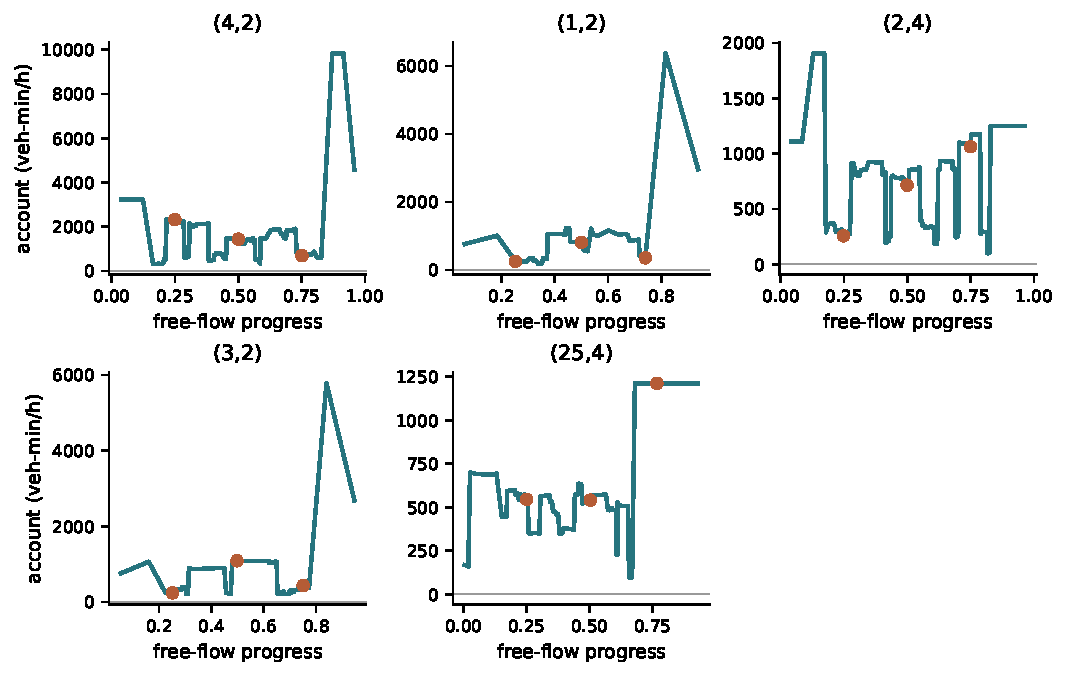
\includegraphics[width=0.99\linewidth]{../figures/fig_v108_anaheim_rest.pdf}
\caption{Anaheim spatial response profiles of the remaining five study
queries over the distance-based families: the attribution versus network-distance
progress along each query's own OD direction, with ochre dots marking
the three prespecified positions. All stay positive; family ranges span
roughly one to one and a half orders of magnitude.}\label{fig:anaheimrest}
\end{figure}
\begin{table}[pos=htbp]\centering\footnotesize\caption{Anaheim attributions over the complete distance-based family, with the three prespecified positions (vehicle-minutes per hour). Column heads are the prespecified targets; the exact selected levels are (row order) $0.250/0.501/0.752$, $0.252/0.500/0.740$, $0.248/0.499/0.750$, $0.251/0.498/0.751$, $0.251/0.504/0.768$ and $0.250/0.500/0.724$.}\label{tab:anaheim}\begin{tabular}{lrrrrrrr}\toprule OD & System & Unrestricted range & Family range & Regions & $\phi(0.25)$ & $\phi(0.50)$ & $\phi(0.75)$\\\midrule
(4,2) & 34664.1 & [-12712.6,20514.0] & [307.5,9832.1] & 211 & 2323.5 & 1441.8 & 692.3\\
(1,2) & 16773.6 & [-6032.2,9762.0] & [172.7,6374.8] & 83 & 259.0 & 818.0 & 360.5\\
(2,4) & 12143.7 & [-4374.6,6733.0] & [98.7,1905.9] & 211 & 257.0 & 714.6 & 1061.8\\
(3,2) & 14706.7 & [-5613.8,9052.9] & [202.8,5777.4] & 157 & 236.2 & 1087.3 & 434.6\\
(25,4) & 6919.3 & [-1805.3,3091.8] & [96.8,1212.2] & 164 & 545.6 & 540.7 & 1212.2\\
(25,2) & 11445.9 & [-4157.3,6904.5] & [131.8,5751.2] & 84 & 801.5 & 412.0 & 5751.2\\
\bottomrule\end{tabular}\end{table}
\begin{table}[pos=htbp]\centering\footnotesize\caption{Anaheim differences between preselected early and late regions, split by free-flow and congestion weights and study and background responses (vehicle-minutes per hour).}\label{tab:anaheimmechanism}\begin{tabular}{lrrrrr}\toprule OD & Free-flow study & Free-flow background & Congestion study & Congestion background & Total\\\midrule
(4,2) & -416.91 & -8.53 & -1499.94 & 294.16 & -1631.21\\
(1,2) & 9.85 & 6.96 & 83.01 & 1.71 & 101.54\\
(2,4) & 312.07 & -65.41 & 667.06 & -108.90 & 804.83\\
(3,2) & 50.04 & 11.80 & 136.55 & 0.04 & 198.43\\
(25,4) & 47.28 & -40.11 & 666.28 & -6.89 & 666.56\\
(25,2) & -131.77 & -10.52 & 5102.23 & -10.15 & 4949.79\\
\bottomrule\end{tabular}\end{table}

\begin{table}[pos=htbp]\centering\footnotesize
\caption{Location layer of the $(25,2)$ case: the boundary at each
reported position, its crossing links, and the principal signed
attribution contributions (vehicle-minutes per hour; positive entries
add to the origin-side attribution). Regions contain the origin; the two
plateau endpoints share the attribution $5{,}751.2$ on link
$63\!\to\!62$, while their second crossing link differs ($87\!\to\!86$
at the start, $2\!\to\!87$ at the end, contributing $-0.0$ at
both).}\label{tab:anaheimcrossing}
\setlength{\tabcolsep}{4pt}
\begin{tabular*}{\tblwidth}{@{\extracolsep{\fill}}lrrrl}
\toprule
Position & Region & Crossing & Principal links & Attribution\\
(progress) & (nodes) & links & (from$\to$to, contribution) &\\
\midrule
Early $0.250$ & 231 & 34 & $269\!\to\!261$ $+550.5$;\ $271\!\to\!192$ $+163.9$ & $801.5$\\
Middle $0.500$ & 405 & 4 & $191\!\to\!190$ $+297.0$;\ $66\!\to\!65$ $+105.4$ & $412.0$\\
Plateau $0.724$--$0.818$ & 413--414 & 2 & $63\!\to\!62$ $+5{,}751.2$;\ ($87\!\to\!86$/$2\!\to\!87$ $-0.0$) & $5{,}751.2$\\
Destination $0.911$ & 415 & 2 & $62\!\to\!2$ $+2{,}673.1$;\ ($2\!\to\!87$ $-0.0$) & $2{,}673.1$\\
\bottomrule\end{tabular*}\end{table}
